\documentclass[8pt,a4paper,compress]{beamer}

\usepackage{/home/siyer/lib/slides}

\title{Elementary Sorts}
\date{}

\begin{document}
\begin{frame}
\vfill
\titlepage
\end{frame}

\begin{frame}
\frametitle{Outline}
\tableofcontents
\end{frame}

\section{Rules of the Game}
\begin{frame}[fragile]
\begin{itemize}
\item sorting is the process of rearranging a sequence of objects so as to put them in some logical order

\item for example, your credit card bill presents transactions ordered by date

\item as a conservative practice, we include the statement \lstinline{assert isSorted(a)} in our test client to certify that array entries are in order after the sort

\item we test algorithm performance by counting the number of basic
operations (comparisons and exchanges or array accesses)

\item there are two types of sorting algorithms: those that sort in place and use no extra memory, and those that need enough extra memory to hold another copy of the array to be sorted

\item our sort code is effective for any item type that implements the \lstinline{Comparable} interface
\end{itemize}
\end{frame}

\begin{frame}[fragile]
\begin{itemize}
\item sort template
\begin{lstlisting}[language=Java]
public class SortAlgorithm {
    public static void sort(Comparable[] a) { ... }
    
    private static boolean less(Comparable v , Comparable w) {
        return (v.compareTo(w) < 0);
    }
    
    private static void exch(Object[] a, int i, int j) {
        Object swap = a[i]; a [i] = a[j]; a[j] = swap;
    }
    
    private static boolean isSorted(Comparable[] a) {
        for (int i = 1; i < a.length; i++) {
            if (less(a[i], a[i - 1])) { return false; }
        }
        return true;
    }
    
    private static void show(Comparable[] a) {
        for (int i = 0; i < a.length ; i++) { StdOut.print(a[i] + " "); }
        StdOut.println();
    }
    
    public static void main(String[] args) {
        String[] a = StdIn.readAllStrings();
        sort(a);
        assert isSorted(a);
        show(a);
    }
}
\end{lstlisting}

\begin{lstlisting}[language={}]
$ echo "S O R T E X A M P L E" | java SortAlgorithm
A E E L M O P R S T X
\end{lstlisting}
\end{itemize}
\end{frame}

\section{Selection Sort}
\begin{frame}[fragile]
\begin{itemize}
\item first find the smallest item in the array and exchange it with the first entry (itself if the first entry is already the smallest), then find the next smallest item and exchange it with the second entry, and so on until the entire array is sorted
\begin{lstlisting}[language=Java]
public class Selection {
    ...
    public static void sort(Comparable[] a) {
        int N = a.length;
        for (int i = 0; i < N; i++) {
            int min = i;
            for (int j = i + 1; j < N; j++) {
                if (less(a[j], a[min])) { 
                    min = j;
                }
            }
            exch(a, i, min);
        }
    }
    ...
}
\end{lstlisting}
\end{itemize}
\end{frame}

\begin{frame}[fragile]
\begin{itemize}
\item trace

\begin{center}
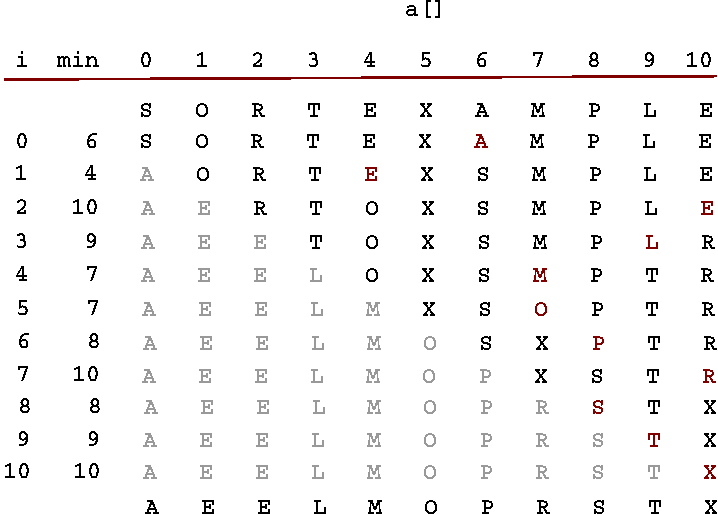
\includegraphics[scale=0.65]{./figures/selection_trace.pdf}

\smallskip

array contents just before each exchange
\end{center}
\end{itemize}
\end{frame}

\begin{frame}[fragile]
\begin{itemize}
\item selection sort uses $\sim N^2/2$ comparisons and $N$ exchanges to sort an array of length $N$

\item it takes about as long to run selection sort for an
array that is already in order or for an array with all keys equal as it does for a randomly-ordered array

\item each of the $N$ exchanges changes the value of two array
entries, so the number of array accesses is a linear function of the array size, a property that none of the other sorting algorithms that we consider have (most involve linearithmic or quadratic growth)
\end{itemize}
\end{frame}

\section{Insertion Sort}
\begin{frame}[fragile]
\begin{itemize}
\item similar to the technique that people use to sort bridge hands, ie, consider the cards one at a time, inserting each into its proper place among those already considered (keeping them sorted)
\begin{lstlisting}[language=Java]
public class Insertion {
    ...
    public static void sort(Comparable[] a) {
        int N = a.length;
        for (int i = 0; i < N; i++) {
            for (int j = i; j > 0 && less(a[j], a[j - 1]); j--) {
                exch(a, j, j - 1);
            }
        }
    }
    ...
}
\end{lstlisting}
\end{itemize}
\end{frame}

\begin{frame}[fragile]
\begin{itemize}
\item trace

\begin{center}
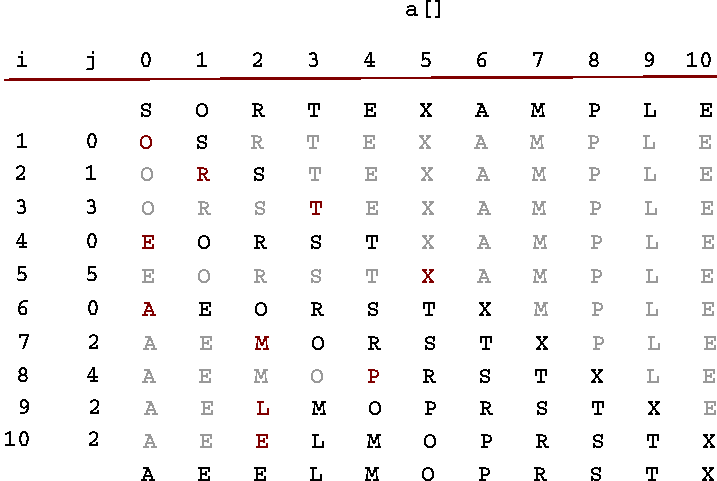
\includegraphics[scale=0.65]{./figures/insertion_trace.pdf}

\smallskip

array contents just after each iteration of the inner loop
\end{center}
\end{itemize}
\end{frame}

\begin{frame}[fragile]
\begin{itemize}
\item insertion sort uses $\sim N^2 /4$ comparisons and $\sim N^2 /4$ exchanges to sort a randomly ordered array of length $N$ with distinct keys, on the average; the worst case is $\sim N^2 /2$ comparisons and $\sim N^2/2$ exchanges; the best case is $N-1$ comparisons and 0 exchanges

\item insertion sort is an excellent method for partially-sorted arrays and is also a fine method for tiny arrays
\end{itemize}
\end{frame}

\section{Shell Sort}
\begin{frame}[fragile]
\begin{itemize}
\item shell sort is a simple extension of insertion sort that gains speed by allowing exchanges of array entries that are far apart, to produce partially-sorted arrays that can be efficiently sorted, eventually by insertion sort

\item the idea is to rearrange the array such that taking every $h$th entry (starting anywhere) yields an $h$-sorted subsequence
\begin{lstlisting}[language=Java]
public class Shell {
    ...
    public static void sort(Comparable[] a) {
        int N = a.length; 
        int h = 1;
        while (h < N / 3) { h = 3 * h + 1; }
        while (h >= 1) {
            for (int i = h; i < N; i++) {
                for (int j = i; j >= h && less(a[j], a[j - h]); j -= h) {
                    exch(a, j, j - h);
                }
            }
            h /= 3;
        }    
    }
    ...
}
\end{lstlisting}
\end{itemize}
\end{frame}

\begin{frame}[fragile]
\begin{itemize}
\item trace

\begin{center}
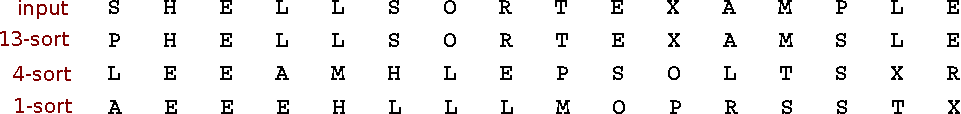
\includegraphics[scale=0.6]{./figures/shell_trace.pdf}

\smallskip

array contents after each pass
\end{center}

\item the worst-case number of comparisons is proportional to $N^{3/2}$; no mathematical results are available for the average-case number of comparisons for randomly ordered input
\end{itemize}
\end{frame}

\section{Visualizing Sorting Algorithms}
\begin{frame}[fragile]
\begin{itemize}
\item using animations

\bigskip

\begin{center}
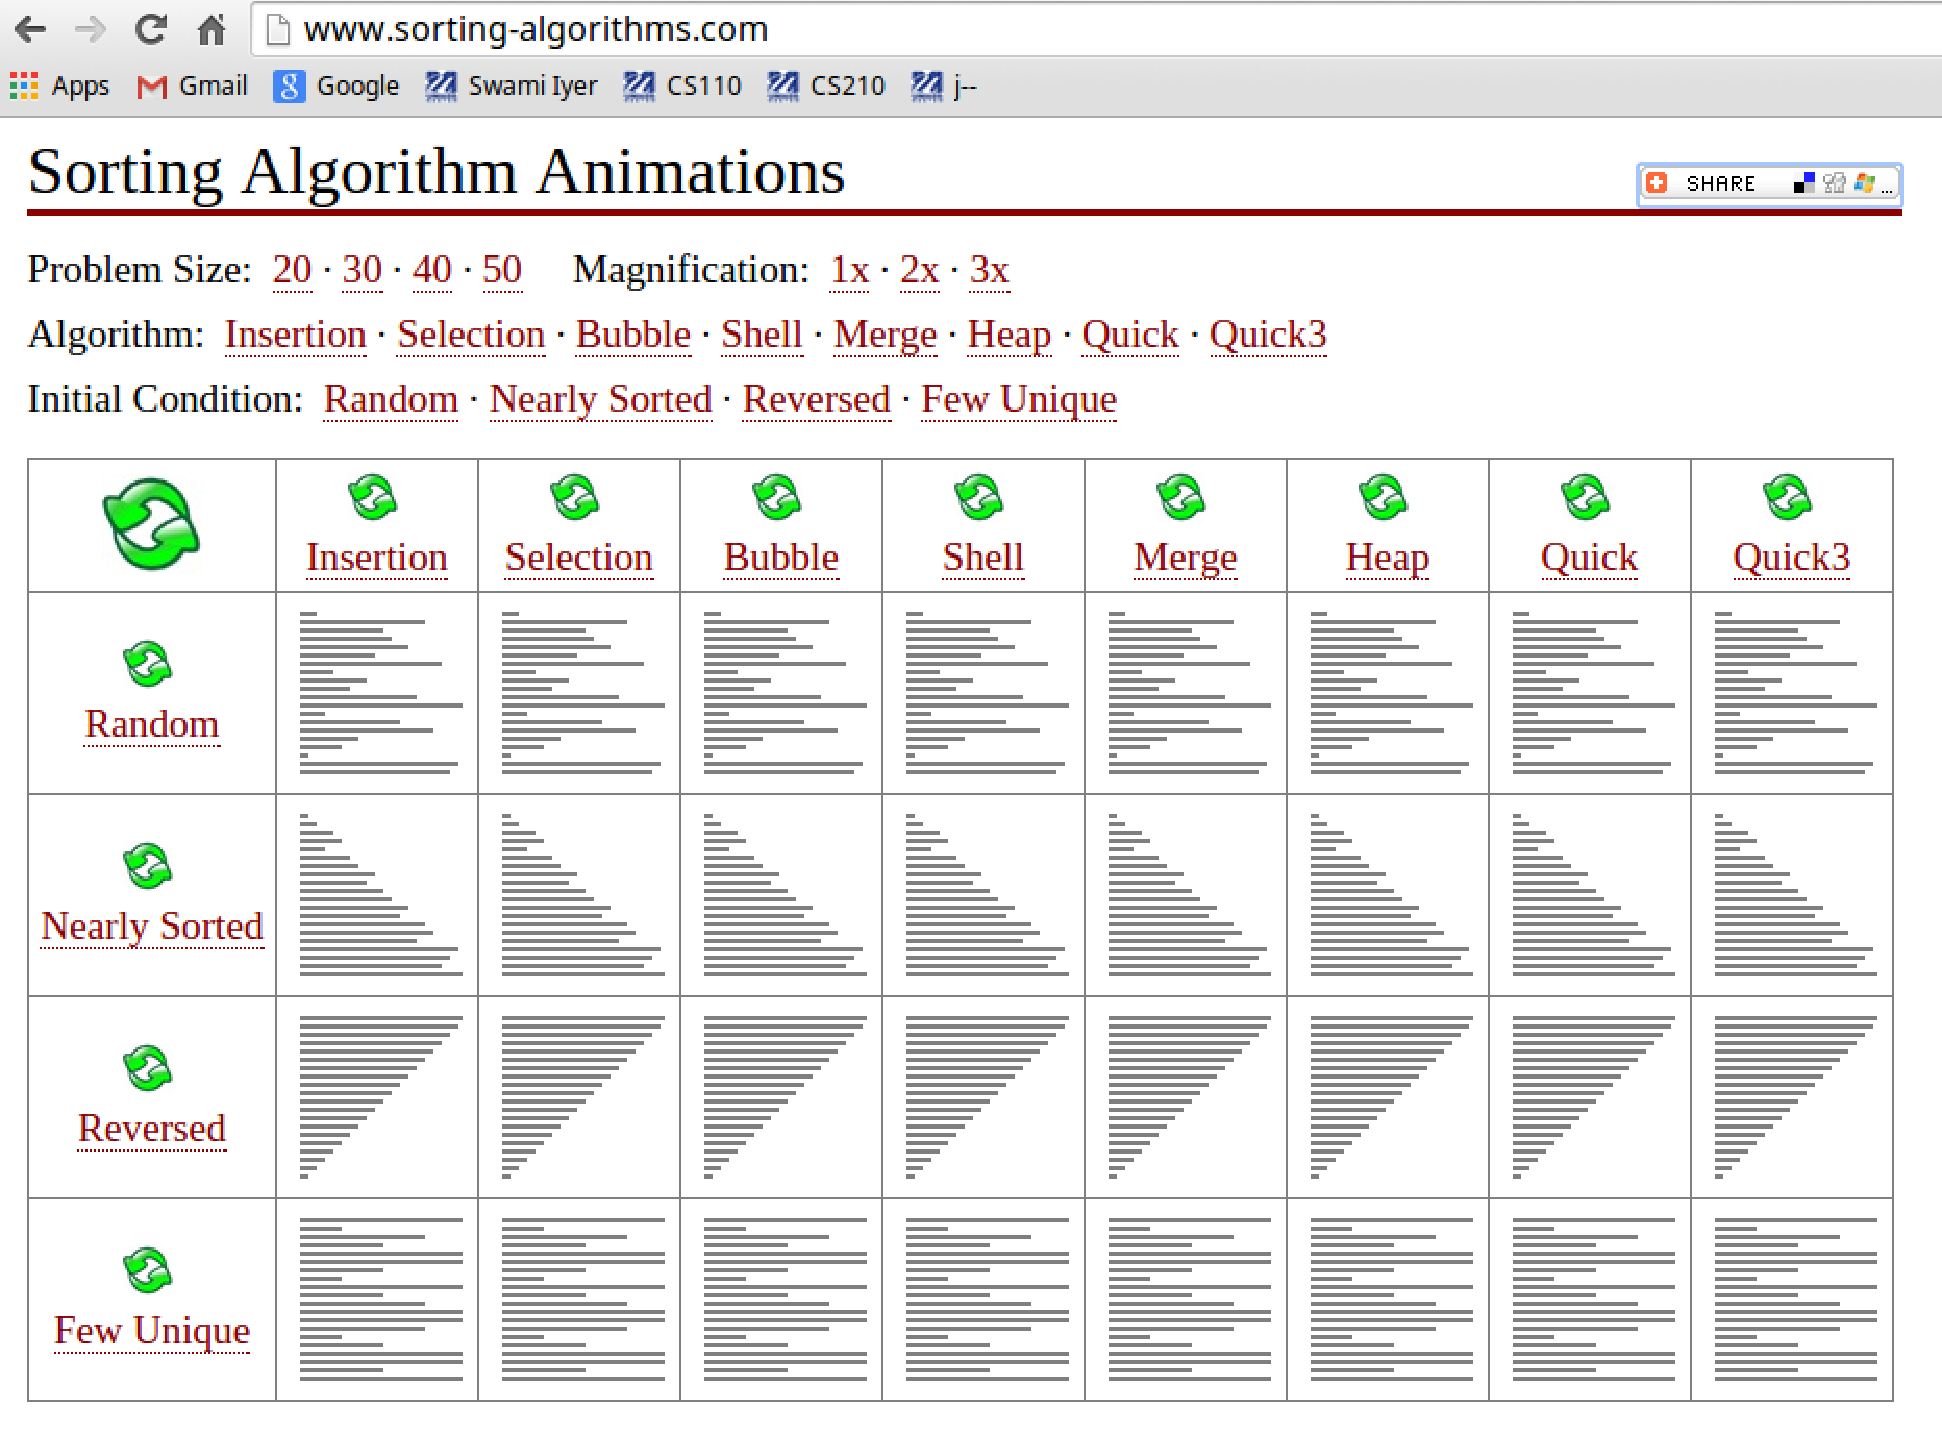
\includegraphics[scale=0.3]{./figures/algorithm_animations.pdf}
\end{center}
\end{itemize}
\end{frame}

\begin{frame}[fragile]
\begin{itemize}
\item using folk dances

\bigskip

\begin{center}
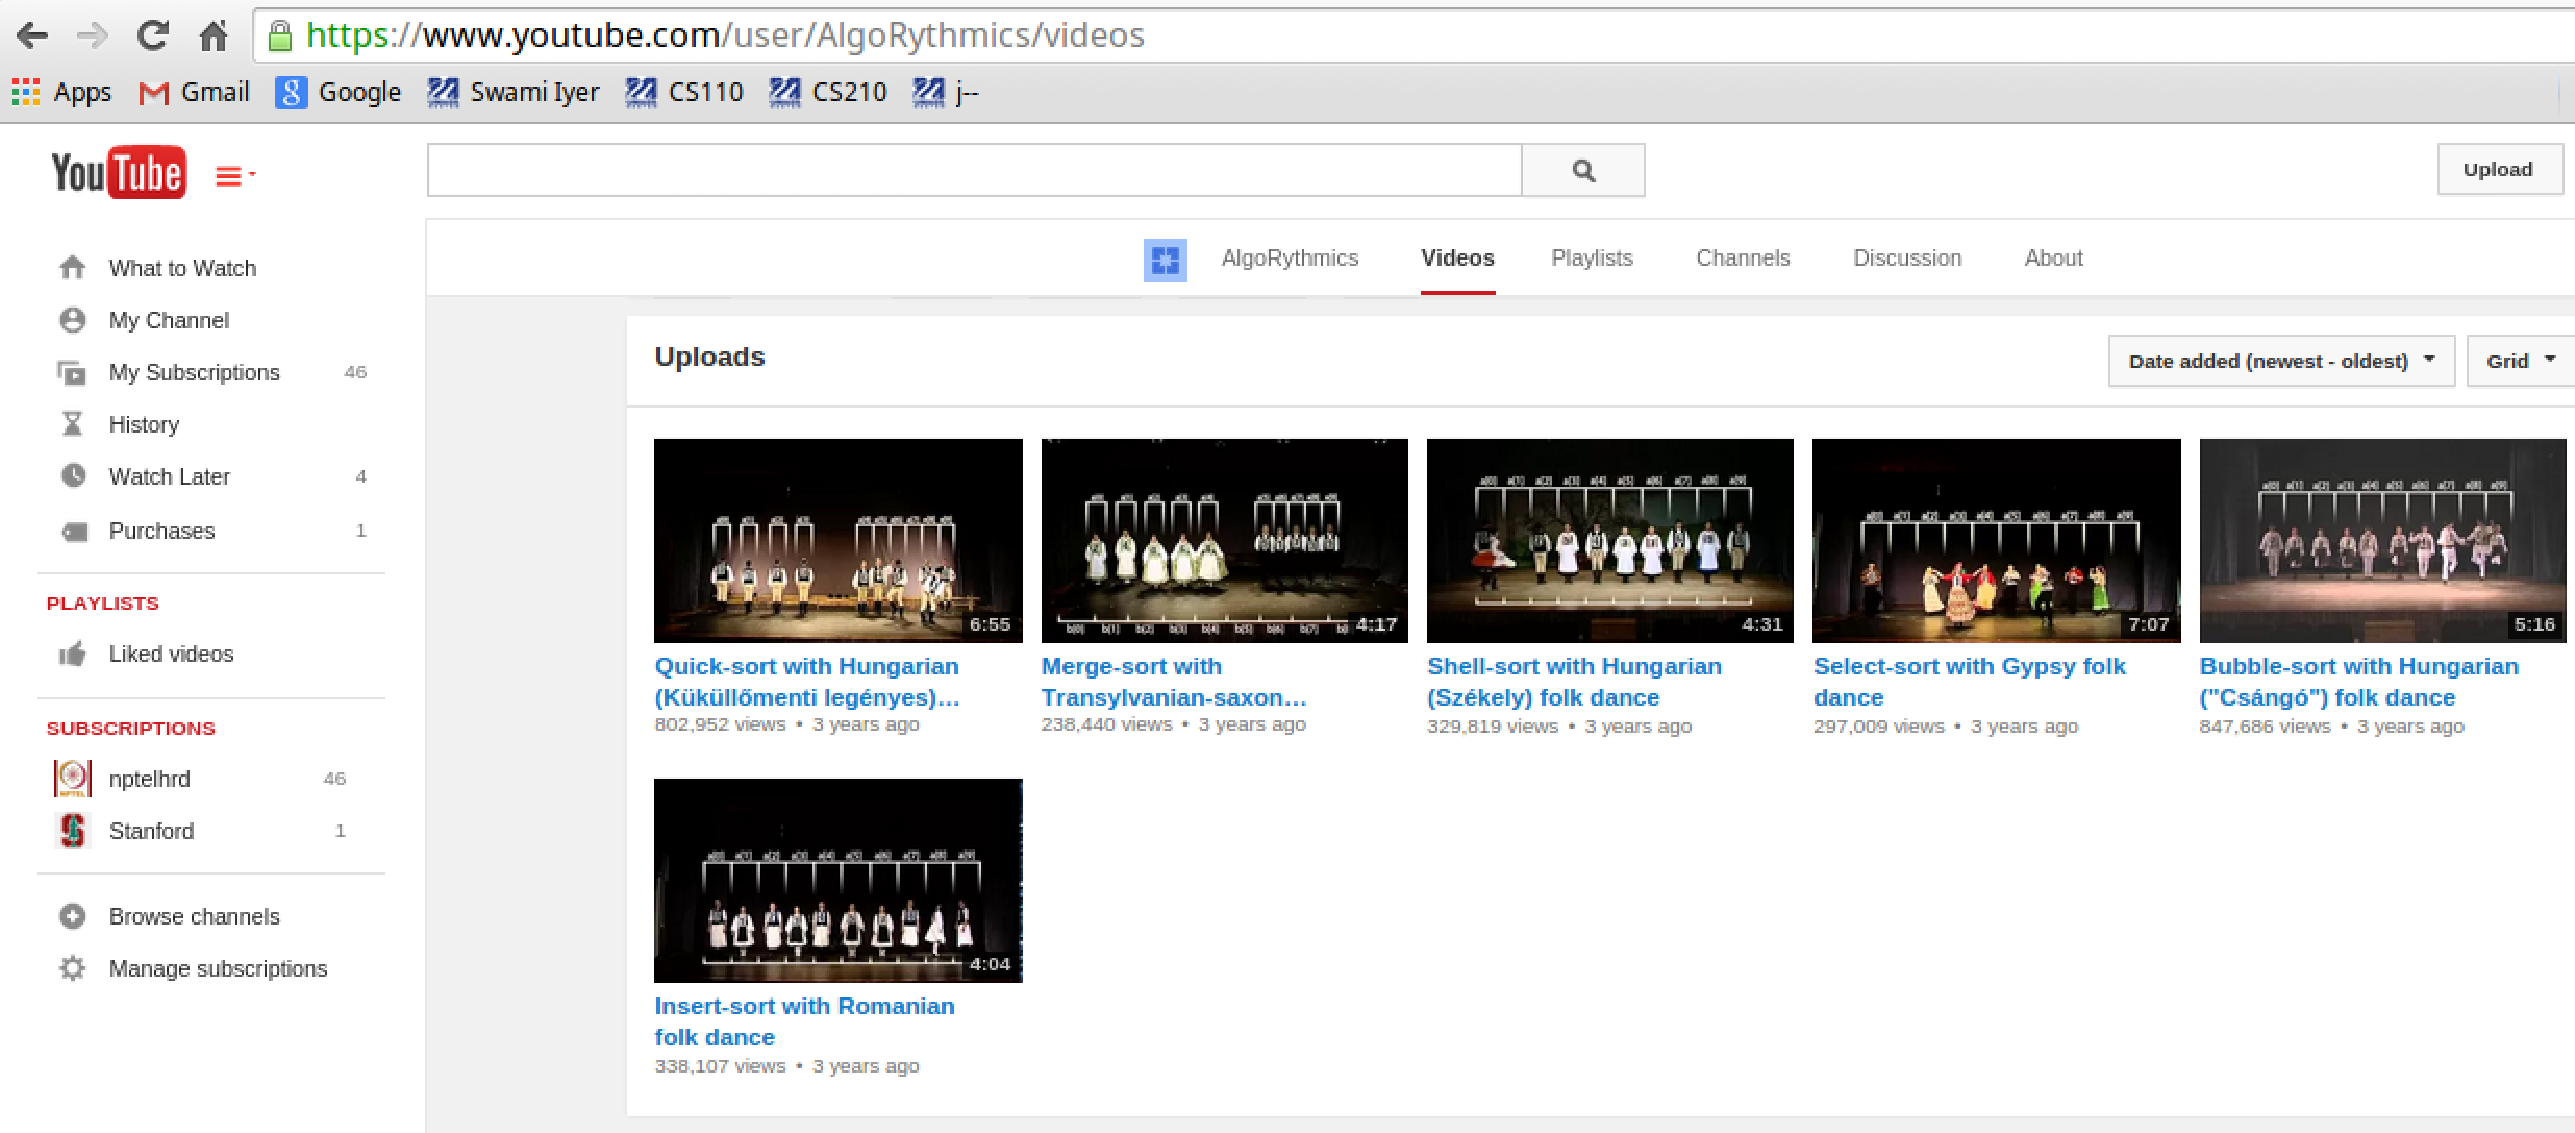
\includegraphics[scale=0.23]{./figures/algorithm_videos.pdf}
\end{center}
\end{itemize}
\end{frame}

\section{Comparing Sorting Algorithms}
\begin{frame}[fragile]
\begin{itemize}
\item \lstinline{SortCompare}
\begin{lstlisting}[language=Java]
import java.util.Arrays;

public class SortCompare { 
    public static double time(String alg, Double[] a) { 
        Stopwatch sw = new Stopwatch(); 
        if (alg.equals("Insertion"))       { Insertion.sort(a); }
        else if (alg.equals("InsertionX")) { InsertionX.sort(a); }
        else if (alg.equals("Selection"))  { Selection.sort(a); }
        else if (alg.equals("Shell"))      { Shell.sort(a); }
        else if (alg.equals("Merge"))      { Merge.sort(a); }
        else if (alg.equals("MergeX"))     { MergeX.sort(a); }
        else if (alg.equals("MergeBU"))    { MergeBU.sort(a); } 
        else if (alg.equals("Quick"))      { Quick.sort(a); }
        else if (alg.equals("Quick3way"))  { Quick3way.sort(a); }
        else if (alg.equals("QuickX"))     { QuickX.sort(a); }
        else if (alg.equals("Heap"))       { Heap.sort(a); }
        else if (alg.equals("System"))     { Arrays.sort(a); }
        else {
            throw new IllegalArgumentException("Invalid algorithm: " + alg);
        }
        return sw.elapsedTime(); 
    } 

    public static double timeRandomInput(String alg, int N, int T)  {
        double total = 0.0; 
        Double[] a = new Double[N]; 
        for (int t = 0; t < T; t++) {
            for (int i = 0; i < N; i++) { a[i] = StdRandom.uniform(); }
            total += time(alg, a); 
        } 
        return total; 
    }
    ... 
}
\end{lstlisting}
\end{itemize}
\end{frame}

\begin{frame}[fragile]
\begin{itemize}
\item \lstinline{SortCompare} (contd.)
\begin{lstlisting}[language=Java]
    ...
    public static void main(String[] args) { 
        String alg1 = args[0]; 
        String alg2 = args[1]; 
        int N = Integer.parseInt(args[2]); 
        int T = Integer.parseInt(args[3]); 
        double time1 = timeRandomInput(alg1, N, T); 
        double time2 = timeRandomInput(alg2, N, T); 
        StdOut.printf("For %d random Doubles\n    %s is", N, alg1); 
        StdOut.printf(" %.1f times faster than %s\n", time2 / time1, alg2); 
    } 
}
\end{lstlisting}

\begin{lstlisting}[language={}]
$ java SortCompare Selection Insertion 10000 100
For 10000 random Doubles
    Selection is 0.9 times faster than Insertion
\end{lstlisting}

\begin{lstlisting}[language={}]
$ java SortCompare Insertion Shell 10000 100
For 10000 random Doubles
    Insertion is 0.0 times faster than Shell
\end{lstlisting}

\begin{lstlisting}[language={}]
$ java SortCompare Shell Selection 10000 100
For 10000 random Doubles
    Shell is 52.5 times faster than Selection
\end{lstlisting}
\end{itemize}
\end{frame}
\end{document}
